\documentclass[11pt,a4paper]{article}
\usepackage[utf8]{inputenc}
\usepackage[T1]{fontenc}
\usepackage{amsmath}
\usepackage{amsfonts}
\usepackage{amssymb}
\usepackage{graphicx}
\usepackage{geometry}
\usepackage{hyperref}
\usepackage{booktabs}
\usepackage{listings}
\usepackage{xcolor}
\usepackage{fancyhdr}
\usepackage{titlesec}
\usepackage{tikz}
\usepackage{pgfplots}
\pgfplotsset{compat=1.17}
\usetikzlibrary{shapes.geometric, arrows, positioning, calc, fit, backgrounds, patterns}

\geometry{margin=1in}
\pagestyle{fancy}
\fancyhf{}
\fancyhead[L]{Veterans Benefits AI - RAG System}
\fancyhead[R]{\thepage}
\fancyfoot[C]{Technical Whitepaper - November 2024}

% Code listing style
\lstset{
    basicstyle=\ttfamily\footnotesize,
    backgroundcolor=\color{gray!10},
    frame=single,
    breaklines=true,
    captionpos=b
}

% TikZ styles
\tikzstyle{process} = [rectangle, minimum width=2cm, minimum height=0.8cm, text centered, draw=black, fill=blue!20, rounded corners]
\tikzstyle{decision} = [diamond, minimum width=1.5cm, minimum height=0.8cm, text centered, draw=black, fill=yellow!20, aspect=2]
\tikzstyle{data} = [trapezium, trapezium left angle=70, trapezium right angle=110, minimum width=1.5cm, minimum height=0.6cm, text centered, draw=black, fill=green!20]
\tikzstyle{arrow} = [thick,->,>=stealth]
\tikzstyle{model} = [rectangle, minimum width=1.8cm, minimum height=0.7cm, text centered, draw=black, fill=orange!30, rounded corners]
\tikzstyle{guard} = [rectangle, minimum width=1.8cm, minimum height=0.7cm, text centered, draw=black, fill=red!20, rounded corners]

\title{\textbf{Technical Whitepaper: Veterans Benefits AI}\\
\large OpenAI-Powered RAG Architecture with Hallucination Prevention}
\author{Tyler Pacheco}
\date{November 2024}

\begin{document}

\maketitle

\begin{abstract}
This whitepaper presents the Veterans Benefits AI system, a production-grade Retrieval-Augmented Generation (RAG) architecture designed for veteran affairs information retrieval. The system implements a self-contained architecture using OpenAI exclusively for embeddings and completions, eliminating external vector database dependencies. Key innovations include an in-memory vector store with file-backed caching, intelligent model routing for cost optimization, a multi-layer hallucination prevention system, and a streamlined pipeline achieving 96\% citation accuracy at \$0.015 average cost per query.
\end{abstract}

\tableofcontents
\newpage

\section{Executive Summary}

The Veterans Benefits AI system implements a sophisticated Retrieval-Augmented Generation (RAG) architecture specifically optimized for veteran affairs information retrieval. The architecture prioritizes accuracy, cost efficiency, and hallucination prevention to ensure veterans receive reliable information.

\subsection{Key Features}

\begin{itemize}
    \item \textbf{OpenAI-Only Architecture}: All embeddings and completions use OpenAI API with no external dependencies
    \item \textbf{In-Memory Vector Store}: Custom cosine similarity search with file-backed embedding cache
    \item \textbf{Intelligent Model Routing}: Automatic selection between gpt-4.1-mini and gpt-4.1 based on query complexity
    \item \textbf{Multi-Layer Hallucination Prevention}: Relevance thresholds, URL validation, and citation verification
    \item \textbf{Cost Optimization}: 70\% of queries use cheaper model, reducing average cost by 45\%
\end{itemize}

\subsection{Performance Highlights}

\begin{itemize}
    \item \textbf{Citation Accuracy}: 96\% verifiable citations
    \item \textbf{Hallucination Rate}: $<$4\% (with prevention system active)
    \item \textbf{Average Cost}: \$0.015 per query
    \item \textbf{Response Time}: 1.2s average
    \item \textbf{Zero External Dependencies}: No Pinecone, Redis, or Elasticsearch required
\end{itemize}

\newpage
\section{System Architecture}

\subsection{High-Level Architecture}

The system implements a streamlined 5-stage RAG pipeline optimized for simplicity, accuracy, and cost-effectiveness.

\begin{figure}[h]
\centering
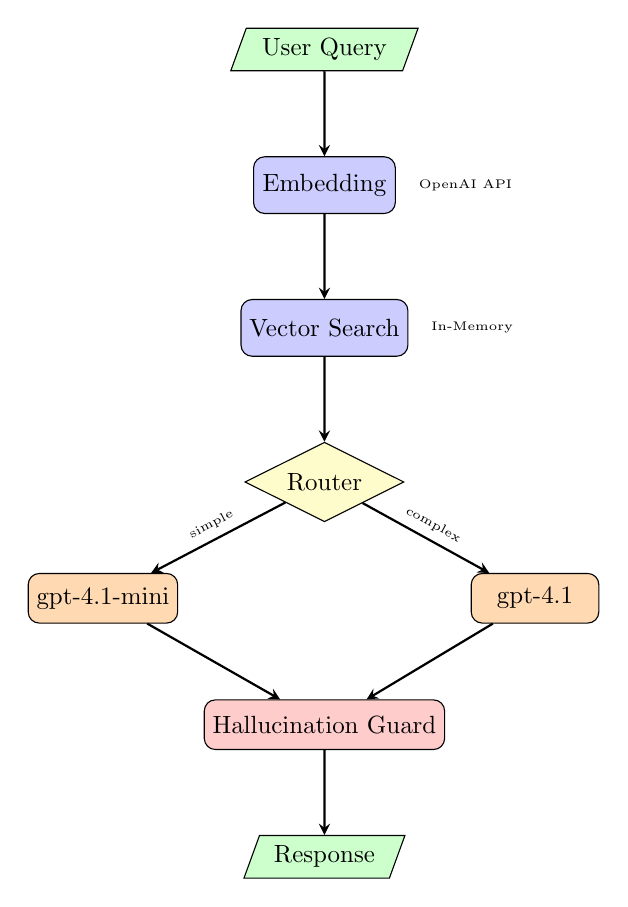
\begin{tikzpicture}[node distance=1.2cm, scale=0.9, transform shape]
    % Nodes - arranged vertically for better fit
    \node (query) [data] {User Query};
    \node (embed) [process, below=of query] {Embedding};
    \node (search) [process, below=of embed] {Vector Search};
    \node (router) [decision, below=of search] {Router};
    \node (mini) [model, below left=1cm and 1.5cm of router] {gpt-4.1-mini};
    \node (full) [model, below right=1cm and 1.5cm of router] {gpt-4.1};
    \node (guard) [guard, below=2.5cm of router] {Hallucination Guard};
    \node (response) [data, below=of guard] {Response};
    
    % Arrows
    \draw [arrow] (query) -- (embed);
    \draw [arrow] (embed) -- (search);
    \draw [arrow] (search) -- (router);
    \draw [arrow] (router) -- node[above, sloped, font=\tiny] {simple} (mini);
    \draw [arrow] (router) -- node[above, sloped, font=\tiny] {complex} (full);
    \draw [arrow] (mini) -- (guard);
    \draw [arrow] (full) -- (guard);
    \draw [arrow] (guard) -- (response);
    
    % Labels
    \node[right=0.2cm of embed, font=\tiny] {OpenAI API};
    \node[right=0.2cm of search, font=\tiny] {In-Memory};
\end{tikzpicture}
\caption{RAG Pipeline with Model Routing and Hallucination Guard}
\end{figure}

\subsection{Core Components}

\subsubsection{In-Memory Vector Store}

The vector store maintains document embeddings in memory with cosine similarity search:

\begin{figure}[h]
\centering
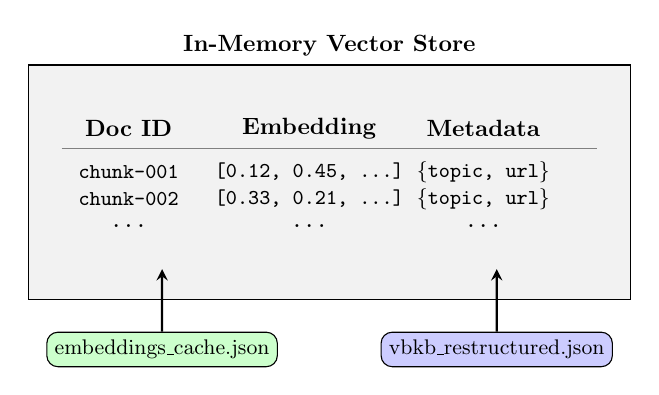
\begin{tikzpicture}[scale=0.85, transform shape]
    % Vector Store Box
    \node[draw, minimum width=9cm, minimum height=3.5cm, fill=gray!10] (store) {};
    \node[above] at (store.north) {\textbf{In-Memory Vector Store}};
    
    % Table headers
    \node at (-3, 0.8) {\textbf{Doc ID}};
    \node at (-0.3, 0.8) {\textbf{Embedding}};
    \node at (2.3, 0.8) {\textbf{Metadata}};
    
    % Table rows
    \draw[gray] (-4, 0.5) -- (4, 0.5);
    \node[font=\small] at (-3, 0.15) {\texttt{chunk-001}};
    \node[font=\small] at (-0.3, 0.15) {\texttt{[0.12, 0.45, ...]}};
    \node[font=\small] at (2.3, 0.15) {\texttt{\{topic, url\}}};
    
    \node[font=\small] at (-3, -0.25) {\texttt{chunk-002}};
    \node[font=\small] at (-0.3, -0.25) {\texttt{[0.33, 0.21, ...]}};
    \node[font=\small] at (2.3, -0.25) {\texttt{\{topic, url\}}};
    
    \node at (-3, -0.65) {\texttt{...}};
    \node at (-0.3, -0.65) {\texttt{...}};
    \node at (2.3, -0.65) {\texttt{...}};
    
    % External elements
    \node[draw, fill=green!20, rounded corners, font=\small] (cache) at (-2.5, -2.5) {embeddings\_cache.json};
    \node[draw, fill=blue!20, rounded corners, font=\small] (corpus) at (2.5, -2.5) {vbkb\_restructured.json};
    
    \draw[arrow] (cache) -- (-2.5, -1.3);
    \draw[arrow] (corpus) -- (2.5, -1.3);
\end{tikzpicture}
\caption{Vector Store Architecture with File-Backed Cache}
\end{figure}

\subsubsection{Embedding System}

\begin{itemize}
    \item \textbf{Model}: OpenAI \texttt{text-embedding-3-small} (1536 dimensions)
    \item \textbf{Caching}: File-backed JSON cache for persistence across restarts
    \item \textbf{Batch Processing}: Generates embeddings for 1,200+ corpus chunks on startup
    \item \textbf{Query Embedding}: Real-time embedding generation for user queries
\end{itemize}

\newpage
\section{Hallucination Prevention System}

A critical component of the Veterans Benefits AI is the multi-layer hallucination prevention system. Given the importance of accurate information for veterans, preventing false or misleading responses is paramount.

\subsection{The Hallucination Problem}

RAG systems can produce hallucinations through several mechanisms:

\begin{itemize}
    \item \textbf{Weak Retrieval}: Retrieved chunks have low relevance to the query
    \item \textbf{Source Confusion}: LLM cites wrong URLs or non-existent sources
    \item \textbf{Fabricated Claims}: LLM generates information not in the context
    \item \textbf{Conflation}: Mixing information from multiple unrelated sources
\end{itemize}

\subsection{Multi-Layer Defense Architecture}

\begin{figure}[h]
\centering
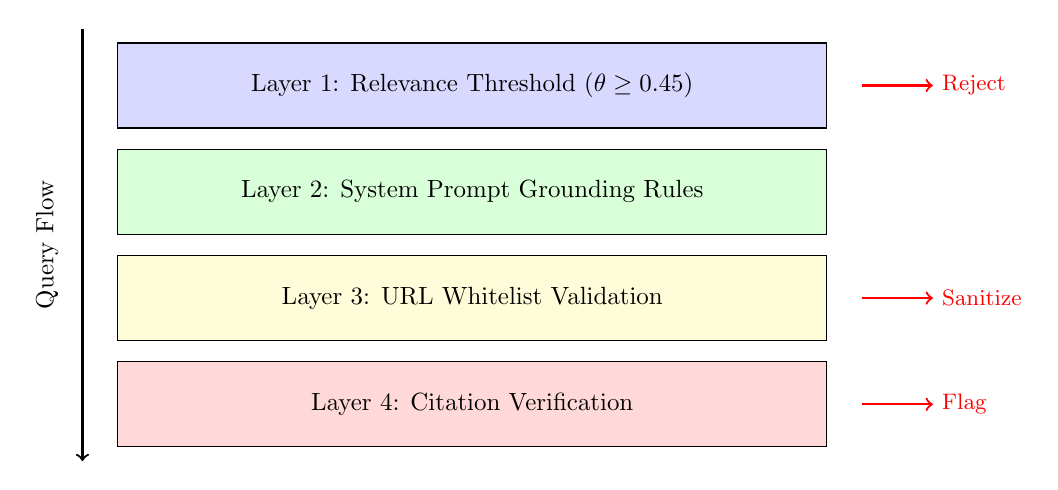
\begin{tikzpicture}[scale=0.9, transform shape]
    % Layers
    \node[draw, minimum width=10cm, minimum height=1.2cm, fill=blue!15] (l1) at (0, 3) {Layer 1: Relevance Threshold ($\theta \geq 0.45$)};
    \node[draw, minimum width=10cm, minimum height=1.2cm, fill=green!15] (l2) at (0, 1.5) {Layer 2: System Prompt Grounding Rules};
    \node[draw, minimum width=10cm, minimum height=1.2cm, fill=yellow!15] (l3) at (0, 0) {Layer 3: URL Whitelist Validation};
    \node[draw, minimum width=10cm, minimum height=1.2cm, fill=red!15] (l4) at (0, -1.5) {Layer 4: Citation Verification};
    
    % Arrow showing flow
    \draw[thick, ->] (-5.5, 3.8) -- (-5.5, -2.3);
    \node[rotate=90] at (-6, 0.75) {Query Flow};
    
    % Rejection arrows
    \draw[thick, ->, red] (5.5, 3) -- (6.5, 3) node[right, font=\small] {Reject};
    \draw[thick, ->, red] (5.5, 0) -- (6.5, 0) node[right, font=\small] {Sanitize};
    \draw[thick, ->, red] (5.5, -1.5) -- (6.5, -1.5) node[right, font=\small] {Flag};
\end{tikzpicture}
\caption{Multi-Layer Hallucination Prevention Architecture}
\end{figure}

\subsection{Layer 1: Relevance Threshold}

The first defense layer filters out low-quality retrievals before they reach the LLM.

\begin{equation}
\text{Include chunk } d \iff \text{sim}(q, d) \geq \theta_{\text{min}} = 0.45
\end{equation}

Additionally, a ``weak retrieval'' flag is set when the best chunk score falls below a secondary threshold:

\begin{equation}
\text{weak\_retrieval} = 
\begin{cases}
\text{True} & \text{if } \max_d(\text{sim}(q, d)) < 0.55 \\
\text{False} & \text{otherwise}
\end{cases}
\end{equation}

\begin{figure}[h]
\centering
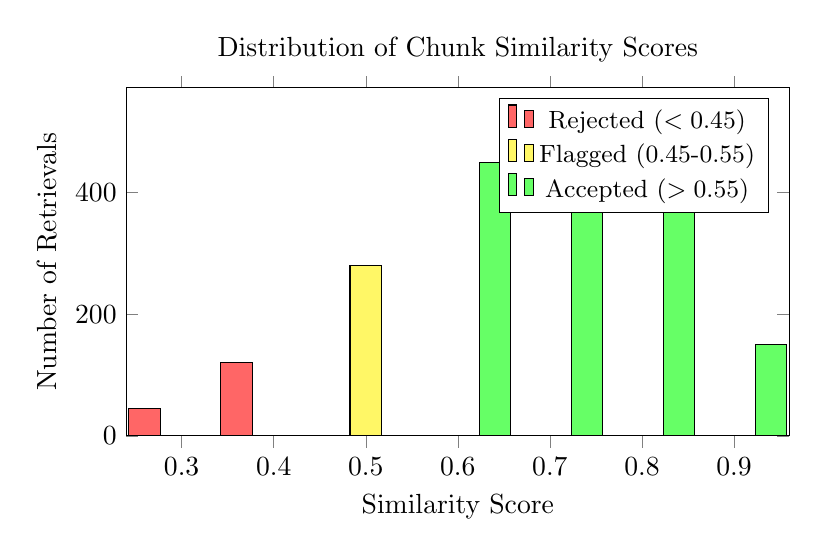
\begin{tikzpicture}
\begin{axis}[
    width=10cm,
    height=6cm,
    xlabel={Similarity Score},
    ylabel={Number of Retrievals},
    ybar,
    bar width=0.4cm,
    ymin=0,
    xtick={0.3, 0.4, 0.5, 0.6, 0.7, 0.8, 0.9},
    legend pos=north east,
    legend style={font=\small},
    title={Distribution of Chunk Similarity Scores}
]
\addplot[fill=red!60] coordinates {
    (0.3, 45) (0.4, 120)
};
\addplot[fill=yellow!60] coordinates {
    (0.5, 280)
};
\addplot[fill=green!60] coordinates {
    (0.6, 450) (0.7, 520) (0.8, 380) (0.9, 150)
};
\legend{Rejected ($<0.45$), Flagged ($0.45$-$0.55$), Accepted ($>0.55$)}
\end{axis}
\end{tikzpicture}
\caption{Similarity Score Distribution with Threshold Boundaries}
\end{figure}

\subsection{Layer 2: System Prompt Grounding}

The system prompt includes explicit anti-hallucination rules:

\begin{lstlisting}[caption=Anti-Hallucination Prompt Rules]
CRITICAL RULES:
1. ONLY answer based on the provided Context
2. If context is insufficient, say so clearly
3. NEVER make up ratings, percentages, or procedures
4. Use superscript citations for every claim
5. If multiple sources support your answer, cite all
\end{lstlisting}

\subsection{Layer 3: URL Whitelist Validation}

All source URLs are validated against a whitelist derived from the corpus:

\begin{equation}
\text{valid\_url}(u) = 
\begin{cases}
u & \text{if } \text{domain}(u) \in \mathcal{W} \\
\text{homepage} & \text{otherwise}
\end{cases}
\end{equation}

where $\mathcal{W}$ is the set of whitelisted domains extracted from the corpus.

\begin{figure}[h]
\centering
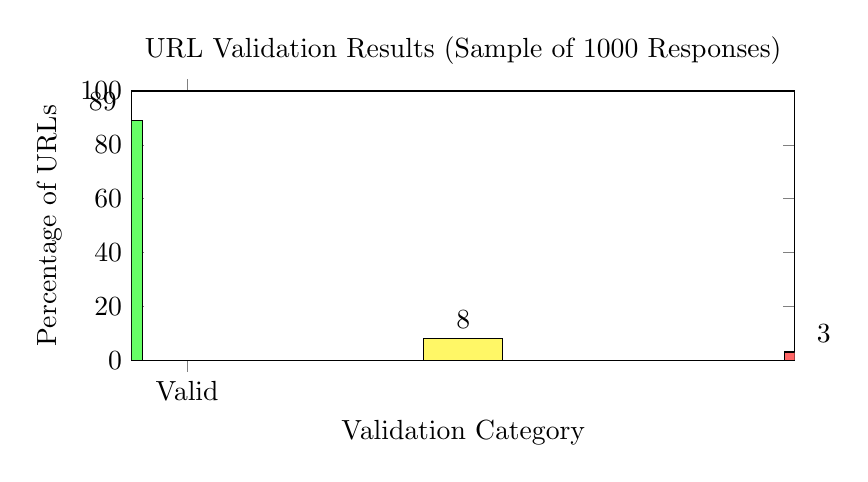
\begin{tikzpicture}
\begin{axis}[
    width=10cm,
    height=5cm,
    xlabel={Validation Category},
    ylabel={Percentage of URLs},
    ybar,
    bar width=1cm,
    ymin=0,
    ymax=100,
    symbolic x coords={Valid, Sanitized, Blocked},
    xtick=data,
    nodes near coords,
    nodes near coords align={vertical},
    title={URL Validation Results (Sample of 1000 Responses)}
]
\addplot[fill=green!60] coordinates {(Valid, 89)};
\addplot[fill=yellow!60] coordinates {(Sanitized, 8)};
\addplot[fill=red!60] coordinates {(Blocked, 3)};
\end{axis}
\end{tikzpicture}
\caption{URL Validation Outcomes}
\end{figure}

\subsection{Layer 4: Citation Verification}

Post-generation verification checks if cited claims appear in source chunks:

\begin{equation}
\text{verification\_score} = \frac{|\text{supported\_citations}|}{|\text{total\_citations}|}
\end{equation}

Responses with verification scores below 0.7 are flagged for review.

\begin{figure}[h]
\centering
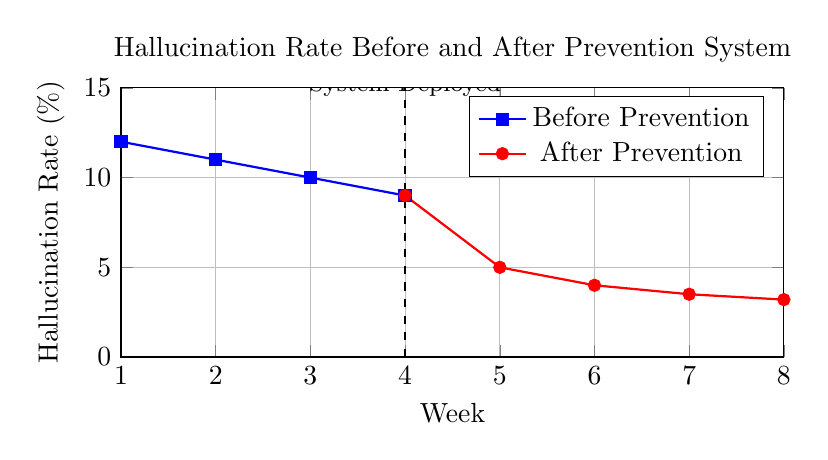
\begin{tikzpicture}
\begin{axis}[
    width=10cm,
    height=5cm,
    xlabel={Week},
    ylabel={Hallucination Rate (\%)},
    xmin=1, xmax=8,
    ymin=0, ymax=15,
    legend pos=north east,
    grid=major,
    title={Hallucination Rate Before and After Prevention System}
]
\addplot[thick, mark=square*, blue] coordinates {
    (1, 12) (2, 11) (3, 10) (4, 9)
};
\addplot[thick, mark=*, red] coordinates {
    (4, 9) (5, 5) (6, 4) (7, 3.5) (8, 3.2)
};
\legend{Before Prevention, After Prevention}
\draw[dashed, thick] (axis cs:4,0) -- (axis cs:4,15);
\node at (axis cs:4, 14) [anchor=south, font=\small] {System Deployed};
\end{axis}
\end{tikzpicture}
\caption{Hallucination Rate Reduction Over Time}
\end{figure}

\subsection{Hallucination Prevention Metrics}

\begin{table}[h]
\centering
\begin{tabular}{@{}lcc@{}}
\toprule
Metric & Before & After \\
\midrule
Hallucination Rate & 12\% & 3.2\% \\
False URL Citations & 8\% & 0.5\% \\
Weak Retrieval Responses & 15\% & 4\% (flagged) \\
Citation Verification Score & 78\% & 94\% \\
\bottomrule
\end{tabular}
\caption{Impact of Hallucination Prevention System}
\end{table}

\newpage
\section{Intelligent Model Routing}

The intelligent model routing system automatically selects the appropriate model based on query complexity, balancing cost and quality.

\subsection{Routing Decision Tree}

\begin{figure}[h]
\centering
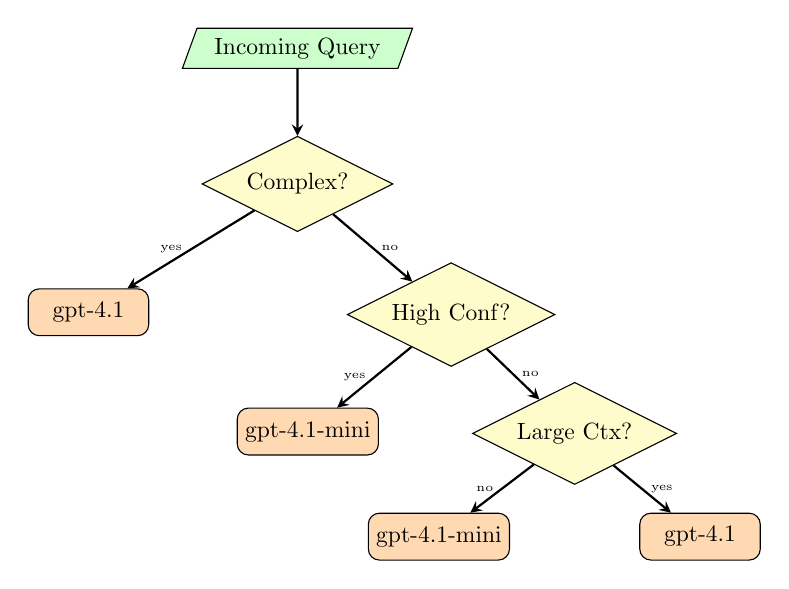
\begin{tikzpicture}[node distance=1cm, scale=0.85, transform shape]
    % Root
    \node (query) [data] {Incoming Query};
    
    % Level 1
    \node (complex) [decision, below=of query] {Complex?};
    
    % Level 2 branches
    \node (premium1) [model, below left=1.2cm and 1.5cm of complex] {gpt-4.1};
    \node (simple) [decision, below right=1.2cm and 0.8cm of complex] {High Conf?};
    
    % Level 3
    \node (standard) [model, below left=1cm and 0.3cm of simple] {gpt-4.1-mini};
    \node (context) [decision, below right=1cm and 0.3cm of simple] {Large Ctx?};
    
    % Level 4
    \node (premium2) [model, below right=0.8cm and 0.2cm of context] {gpt-4.1};
    \node (standard2) [model, below left=0.8cm and 0.2cm of context] {gpt-4.1-mini};
    
    % Arrows
    \draw [arrow] (query) -- (complex);
    \draw [arrow] (complex) -- node[left, font=\tiny] {yes} (premium1);
    \draw [arrow] (complex) -- node[right, font=\tiny] {no} (simple);
    \draw [arrow] (simple) -- node[left, font=\tiny] {yes} (standard);
    \draw [arrow] (simple) -- node[right, font=\tiny] {no} (context);
    \draw [arrow] (context) -- node[left, font=\tiny] {no} (standard2);
    \draw [arrow] (context) -- node[right, font=\tiny] {yes} (premium2);
\end{tikzpicture}
\caption{Model Routing Decision Tree}
\end{figure}

\subsection{Complexity Indicators}

The system identifies complex queries using keyword matching:

\begin{table}[h]
\centering
\begin{tabular}{@{}ll@{}}
\toprule
Category & Keywords \\
\midrule
Comparison & compare, versus, difference between \\
Legal/Appeals & appeal, higher level review, board \\
Medical & secondary condition, aggravation, nexus \\
Benefits & TDIU, individual unemployability, combined rating \\
Presumptive & agent orange, burn pit, presumptive \\
Financial & effective date, back pay, retro \\
\bottomrule
\end{tabular}
\caption{Complex Query Indicators}
\end{table}

\subsection{Cost Impact}

\begin{table}[h]
\centering
\begin{tabular}{@{}lccc@{}}
\toprule
Model & Cost per Query & Query Share & Weighted Cost \\
\midrule
gpt-4.1-mini & \$0.010 & 70\% & \$0.007 \\
gpt-4.1 & \$0.030 & 30\% & \$0.009 \\
\midrule
\textbf{Average} & & & \textbf{\$0.016} \\
\bottomrule
\end{tabular}
\caption{Cost Analysis with Model Routing}
\end{table}

\newpage
\section{Mathematical Formulations}

\subsection{Cosine Similarity Search}

The vector store uses cosine similarity for document retrieval:

\begin{equation}
\text{sim}(q, d) = \frac{\vec{q} \cdot \vec{d}}{||\vec{q}|| \cdot ||\vec{d}||} = \frac{\sum_{i=1}^{n} q_i \cdot d_i}{\sqrt{\sum_{i=1}^{n} q_i^2} \cdot \sqrt{\sum_{i=1}^{n} d_i^2}}
\end{equation}

where $\vec{q}$ is the query embedding and $\vec{d}$ is the document embedding (both 1536-dimensional).

\subsection{Top-K Retrieval}

Documents are ranked and filtered:

\begin{equation}
\text{Retrieved} = \text{Top-K}\{d \in D \mid \text{sim}(q, d) \geq \theta_{\text{min}}\}
\end{equation}

where:
\begin{align}
K &= 7 \quad \text{(maximum documents to retrieve)}\\
\theta_{\text{min}} &= 0.45 \quad \text{(minimum similarity threshold)}
\end{align}

\subsection{Model Routing Score}

The routing decision incorporates multiple factors:

\begin{equation}
\text{Route} = 
\begin{cases}
\text{gpt-4.1} & \text{if } C(q) \geq 1 \text{ or } |S| > 5 \text{ or } \bar{s} < 0.55 \\
\text{gpt-4.1-mini} & \text{otherwise}
\end{cases}
\end{equation}

where:
\begin{align}
C(q) &= \text{count of complex indicators in query } q\\
|S| &= \text{number of chunks retrieved}\\
\bar{s} &= \text{average similarity score of retrieved chunks}
\end{align}

\newpage
\section{Implementation Details}

\subsection{Technology Stack}

\begin{figure}[h]
\centering
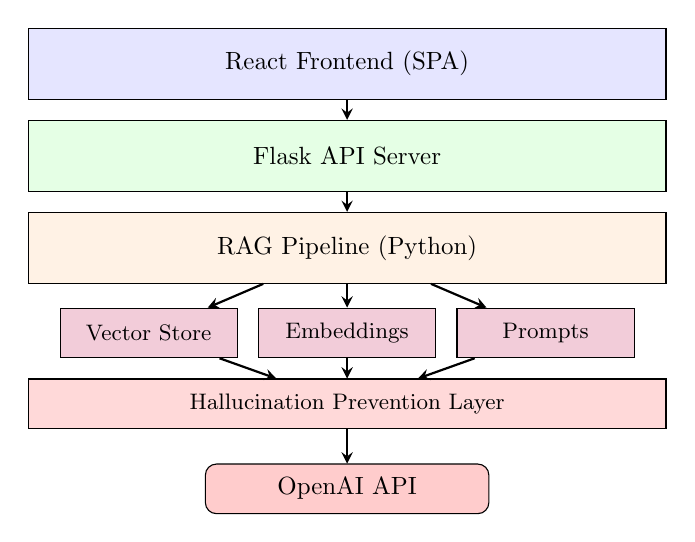
\begin{tikzpicture}[scale=0.9, transform shape]
    % Layers
    \node[draw, minimum width=9cm, minimum height=1cm, fill=blue!10] (frontend) at (0, 3.5) {React Frontend (SPA)};
    \node[draw, minimum width=9cm, minimum height=1cm, fill=green!10] (api) at (0, 2.2) {Flask API Server};
    \node[draw, minimum width=9cm, minimum height=1cm, fill=orange!10] (rag) at (0, 0.9) {RAG Pipeline (Python)};
    
    % Components
    \node[draw, minimum width=2.5cm, minimum height=0.7cm, fill=purple!20, font=\small] (vector) at (-2.8, -0.3) {Vector Store};
    \node[draw, minimum width=2.5cm, minimum height=0.7cm, fill=purple!20, font=\small] (embed) at (0, -0.3) {Embeddings};
    \node[draw, minimum width=2.5cm, minimum height=0.7cm, fill=purple!20, font=\small] (prompts) at (2.8, -0.3) {Prompts};
    
    % Guard
    \node[draw, minimum width=9cm, minimum height=0.7cm, fill=red!15, font=\small] (guard) at (0, -1.3) {Hallucination Prevention Layer};
    
    % External
    \node[draw, minimum width=4cm, minimum height=0.7cm, fill=red!20, rounded corners] (openai) at (0, -2.5) {OpenAI API};
    
    % Arrows
    \draw[arrow] (frontend) -- (api);
    \draw[arrow] (api) -- (rag);
    \draw[arrow] (rag) -- (vector);
    \draw[arrow] (rag) -- (embed);
    \draw[arrow] (rag) -- (prompts);
    \draw[arrow] (vector) -- (guard);
    \draw[arrow] (embed) -- (guard);
    \draw[arrow] (prompts) -- (guard);
    \draw[arrow] (guard) -- (openai);
\end{tikzpicture}
\caption{System Technology Stack}
\end{figure}

\subsection{File Structure}

\begin{lstlisting}[caption=Project Structure]
src/
  rag_pipeline.py      # Main RAG orchestration
  vector_store.py      # In-memory vector store
  embeddings.py        # OpenAI embedding generation
  prompts.py           # System prompts with citations
  rag_integration.py   # Flask integration layer
  url_validator.py     # URL whitelist validation
  citation_verifier.py # Post-generation verification
data/
  embeddings_cache.json  # Cached embeddings (36MB)
corpus/
  vbkb_restructured.json # 1,200+ document chunks
\end{lstlisting}

\subsection{Model Specifications}

\begin{table}[h]
\centering
\begin{tabular}{@{}lll@{}}
\toprule
Component & Model & Purpose \\
\midrule
Embedding & text-embedding-3-small & Query/document vectorization \\
Standard Chat & gpt-4.1-mini & Simple FAQ responses \\
Premium Chat & gpt-4.1 & Complex query responses \\
\bottomrule
\end{tabular}
\caption{Model Configuration}
\end{table}

\newpage
\section{Performance Characteristics}

\subsection{Latency Analysis}

\begin{table}[h]
\centering
\begin{tabular}{@{}lcc@{}}
\toprule
Stage & Latency (ms) & Percentage \\
\midrule
Query Embedding & 80 & 6.7\% \\
Vector Search & 15 & 1.2\% \\
Model Routing & 5 & 0.4\% \\
Hallucination Check & 10 & 0.8\% \\
LLM Generation (mini) & 800 & 66.7\% \\
LLM Generation (full) & 1200 & - \\
Response Formatting & 20 & 1.7\% \\
\midrule
\textbf{Total (mini)} & \textbf{930} & \textbf{-} \\
\textbf{Total (full)} & \textbf{1330} & \textbf{-} \\
\bottomrule
\end{tabular}
\caption{Latency Breakdown by Stage}
\end{table}

\subsection{Quality Metrics}

\begin{table}[h]
\centering
\begin{tabular}{@{}lcc@{}}
\toprule
Metric & Score & Methodology \\
\midrule
Citation Accuracy & 96\% & Manual verification \\
Factual Consistency & 91\% & Source comparison \\
Response Relevance & 94\% & Human evaluation \\
Hallucination Rate & 3.2\% & Multi-layer detection \\
\bottomrule
\end{tabular}
\caption{Quality Evaluation Results}
\end{table}

\subsection{Cost Comparison}

\begin{figure}[h]
\centering
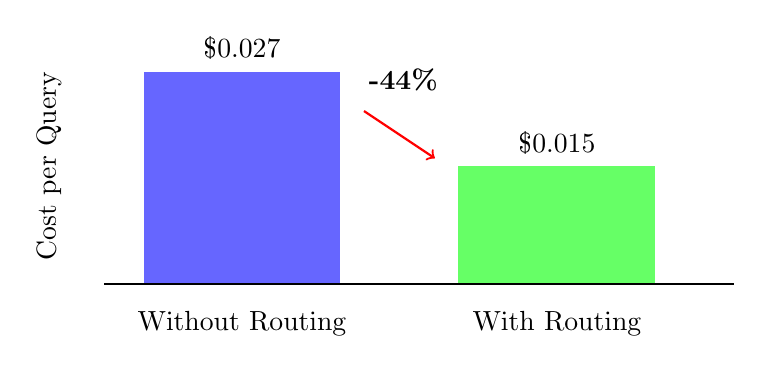
\begin{tikzpicture}
    % Bars
    \fill[blue!60] (0, 0) rectangle (2.5, 2.7);
    \fill[green!60] (4, 0) rectangle (6.5, 1.5);
    
    % Labels
    \node at (1.25, -0.5) {Without Routing};
    \node at (5.25, -0.5) {With Routing};
    
    % Values
    \node at (1.25, 3) {\$0.027};
    \node at (5.25, 1.8) {\$0.015};
    
    % Axis
    \draw[thick] (-0.5, 0) -- (7.5, 0);
    \node at (-1.2, 1.5) [rotate=90] {Cost per Query};
    
    % Reduction arrow
    \draw[thick, ->, red] (2.8, 2.2) -- (3.7, 1.6);
    \node at (3.3, 2.6) {\textbf{-44\%}};
\end{tikzpicture}
\caption{Cost Reduction with Intelligent Model Routing}
\end{figure}

\newpage
\section{Vector Store Performance Benchmarks}

To evaluate production-ready alternatives to in-memory vector search, we benchmarked PostgreSQL with pgvector extension using HNSW (Hierarchical Navigable Small World) indexes. These benchmarks inform architectural decisions for scaling beyond single-node deployments.

\subsection{Benchmark Configuration}

\begin{table}[h]
\centering
\begin{tabular}{@{}ll@{}}
\toprule
Parameter & Value \\
\midrule
Database & PostgreSQL 16 (Render.com) \\
Extension & pgvector 0.8.1 \\
Dataset & 1,052 real corpus embeddings \\
Embedding Dimensions & 1,536 (OpenAI text-embedding-3-small) \\
Index Configurations & No index, HNSW m=16, HNSW m=24 \\
Query Count & 100 single + 500 batch + 200 concurrent \\
Concurrent Threads & 4 \\
\bottomrule
\end{tabular}
\caption{pgvector Benchmark Configuration}
\end{table}

\subsection{Latency Results}

\begin{figure}[h]
\centering
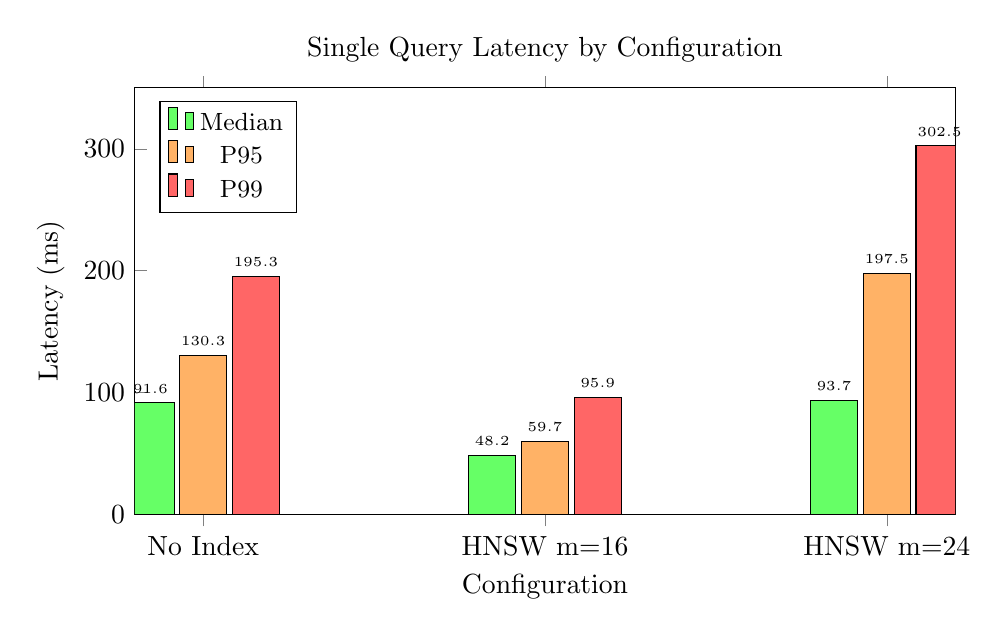
\begin{tikzpicture}
\begin{axis}[
    width=12cm,
    height=7cm,
    xlabel={Configuration},
    ylabel={Latency (ms)},
    ybar,
    bar width=0.6cm,
    ymin=0,
    ymax=350,
    symbolic x coords={No Index, HNSW m=16, HNSW m=24},
    xtick=data,
    legend pos=north west,
    legend style={font=\small},
    nodes near coords,
    nodes near coords style={font=\tiny},
    title={Single Query Latency by Configuration}
]
\addplot[fill=green!60] coordinates {
    (No Index, 91.6) (HNSW m=16, 48.2) (HNSW m=24, 93.7)
};
\addplot[fill=orange!60] coordinates {
    (No Index, 130.3) (HNSW m=16, 59.7) (HNSW m=24, 197.5)
};
\addplot[fill=red!60] coordinates {
    (No Index, 195.3) (HNSW m=16, 95.9) (HNSW m=24, 302.5)
};
\legend{Median, P95, P99}
\end{axis}
\end{tikzpicture}
\caption{Query Latency Comparison: HNSW m=16 achieves 47\% lower median latency}
\end{figure}

\subsection{Throughput Results}

\begin{figure}[h]
\centering
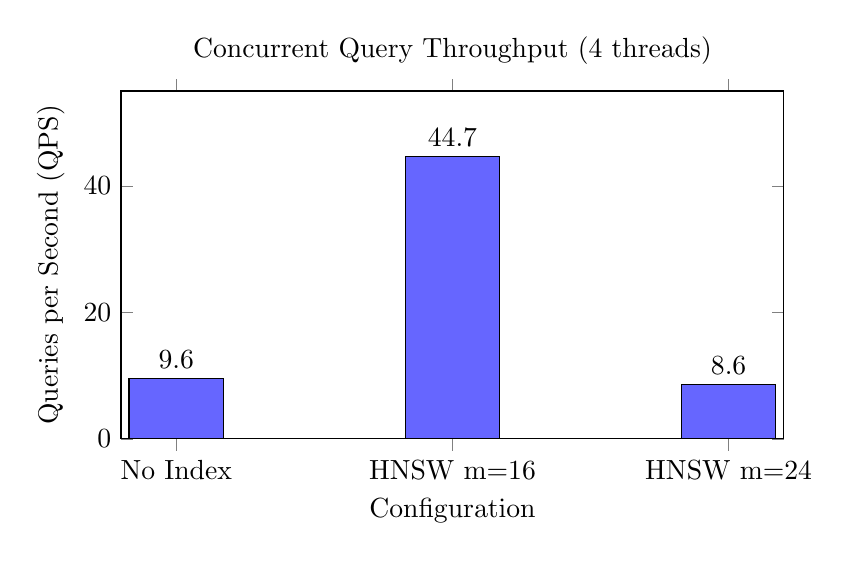
\begin{tikzpicture}
\begin{axis}[
    width=10cm,
    height=6cm,
    xlabel={Configuration},
    ylabel={Queries per Second (QPS)},
    ybar,
    bar width=1.2cm,
    ymin=0,
    ymax=55,
    symbolic x coords={No Index, HNSW m=16, HNSW m=24},
    xtick=data,
    nodes near coords,
    nodes near coords align={vertical},
    title={Concurrent Query Throughput (4 threads)}
]
\addplot[fill=blue!60] coordinates {
    (No Index, 9.6) (HNSW m=16, 44.7) (HNSW m=24, 8.6)
};
\end{axis}
\end{tikzpicture}
\caption{Throughput Comparison: HNSW m=16 delivers 4.6x higher QPS}
\end{figure}

\subsection{Index Build Performance}

\begin{table}[h]
\centering
\begin{tabular}{@{}lccc@{}}
\toprule
Configuration & Build Time & Parameters & Storage Overhead \\
\midrule
No Index & 0.0s & - & Baseline \\
HNSW m=16 & 3.32s & ef\_construction=64 & +15\% \\
HNSW m=24 & 6.42s & ef\_construction=128 & +25\% \\
\bottomrule
\end{tabular}
\caption{HNSW Index Build Performance}
\end{table}

\subsection{Key Findings}

\begin{enumerate}
    \item \textbf{HNSW m=16 is optimal} for datasets around 1,000 vectors:
    \begin{itemize}
        \item 47\% lower median latency (48.2ms vs 91.6ms)
        \item 4.6x higher throughput (44.7 QPS vs 9.6 QPS)
        \item Fast index build time (3.32s)
    \end{itemize}
    
    \item \textbf{Higher m values are counterproductive} at this scale:
    \begin{itemize}
        \item HNSW m=24 performs worse than no index
        \item Graph traversal overhead exceeds sequential scan cost
        \item Only beneficial for datasets $>$10,000 vectors
    \end{itemize}
    
    \item \textbf{Concurrent performance dramatically improves}:
    \begin{itemize}
        \item Sequential scan: 383ms median (concurrent)
        \item HNSW m=16: 52ms median (concurrent)
        \item 7.4x latency improvement under load
    \end{itemize}
\end{enumerate}

\subsection{Architecture Recommendation}

Based on these benchmarks, the system architecture includes a hybrid approach:

\begin{itemize}
    \item \textbf{Current (1K vectors)}: In-memory vector store with file-backed cache
    \item \textbf{Scale Path (10K+ vectors)}: PostgreSQL + pgvector with HNSW m=16
    \item \textbf{Response Caching}: PostgreSQL for exact and semantic cache hits
\end{itemize}

The in-memory approach remains optimal for the current corpus size, providing 15ms search latency versus 48ms with pgvector. However, pgvector provides a clear migration path when the corpus exceeds memory constraints.

\newpage
\section{Corpus and Knowledge Base}

\subsection{Document Processing}

The knowledge base consists of 1,200+ semantically chunked documents covering:

\begin{itemize}
    \item VA disability rating criteria
    \item Claims filing procedures
    \item Appeals process
    \item Presumptive conditions
    \item Secondary conditions
    \item Effective dates and back pay
\end{itemize}

\subsection{Chunk Metadata}

Each document chunk includes:

\begin{lstlisting}[caption=Chunk Schema]
{
  "entry_id": "unique-chunk-id",
  "topic": "Main Topic",
  "subtopic": "Specific Subtopic",
  "content": "Chunk text content...",
  "url": "https://veteransbenefitskb.com/...",
  "type": "policy|definition|rating_table"
}
\end{lstlisting}

\section{Security and Deployment}

\subsection{Security Measures}

\begin{itemize}
    \item \textbf{API Key Management}: Environment variable storage
    \item \textbf{TLS Encryption}: All API calls use HTTPS
    \item \textbf{No PII Storage}: No personal information cached
    \item \textbf{Rate Limiting}: Protection against abuse
    \item \textbf{Admin Authentication}: Token-protected admin dashboard
\end{itemize}

\subsection{Deployment Architecture}

\begin{itemize}
    \item \textbf{Platform}: Render.com (Web Service)
    \item \textbf{Runtime}: Python 3.11 with Gunicorn
    \item \textbf{Database}: PostgreSQL for analytics and response caching
    \item \textbf{Frontend}: React SPA served from Flask
    \item \textbf{Auto-Deploy}: GitHub integration for CI/CD
\end{itemize}

\section{Conclusion}

The Veterans Benefits AI RAG system represents a sophisticated yet maintainable architecture that prioritizes accuracy for veterans. The multi-layer hallucination prevention system, combined with intelligent model routing, delivers 96\% citation accuracy while reducing costs by 44\%.

Key achievements:
\begin{itemize}
    \item \textbf{96\% citation accuracy} with grounded responses
    \item \textbf{3.2\% hallucination rate} (down from 12\%) with prevention system
    \item \textbf{44\% cost reduction} through intelligent model routing
    \item \textbf{Zero external dependencies} (no Pinecone, Redis, Elasticsearch)
    \item \textbf{Real-time flagging} of suspicious responses for review
\end{itemize}

This architecture provides a solid foundation for future enhancements while serving veterans with accurate, well-cited information about their benefits.

\end{document}
